% LLM-Based Summarization - BSc Discovery Redesign
% Complete 36-slide presentation with discovery-based pedagogy
% Target audience: Undergraduate students (BSc level)
% Focus: Technical architecture and advanced techniques (RAG, CoT)
% Template: Madrid theme with BSc Discovery color scheme

\documentclass[8pt,aspectratio=169]{beamer}
\usetheme{Madrid}
\usepackage{graphicx}
\usepackage{booktabs}
\usepackage{adjustbox}
\usepackage{multicol}
\usepackage{amsmath}
\usepackage{tikz}
\usepackage{array}
\usepackage{listings}
\usepackage{algorithm2e}
\usepackage{tabularx}
\usepackage{multirow}
\usepackage{subcaption}

% Color definitions (BSc Discovery theme)
\definecolor{mlblue}{RGB}{0,102,204}
\definecolor{mlpurple}{RGB}{51,51,178}
\definecolor{mllavender}{RGB}{173,173,224}
\definecolor{mllavender2}{RGB}{193,193,232}
\definecolor{mllavender3}{RGB}{204,204,235}
\definecolor{mllavender4}{RGB}{214,214,239}
\definecolor{mlorange}{RGB}{255, 127, 14}
\definecolor{mlgreen}{RGB}{44, 160, 44}
\definecolor{mlred}{RGB}{214, 39, 40}
\definecolor{mlgray}{RGB}{127, 127, 127}
\definecolor{lightgray}{RGB}{240, 240, 240}
\definecolor{midgray}{RGB}{180, 180, 180}

% Apply custom colors to Madrid theme
\setbeamercolor{palette primary}{bg=mllavender3,fg=mlpurple}
\setbeamercolor{palette secondary}{bg=mllavender2,fg=mlpurple}
\setbeamercolor{palette tertiary}{bg=mllavender,fg=white}
\setbeamercolor{palette quaternary}{bg=mlpurple,fg=white}

\setbeamercolor{structure}{fg=mlpurple}
\setbeamercolor{section in toc}{fg=mlpurple}
\setbeamercolor{subsection in toc}{fg=mlblue}
\setbeamercolor{title}{fg=mlpurple}
\setbeamercolor{frametitle}{fg=mlpurple,bg=mllavender3}
\setbeamercolor{block title}{bg=mllavender2,fg=mlpurple}
\setbeamercolor{block body}{bg=mllavender4,fg=black}

% Remove navigation symbols
\setbeamertemplate{navigation symbols}{}

% Clean itemize/enumerate
\setbeamertemplate{itemize items}[circle]
\setbeamertemplate{enumerate items}[default]

% Reduce margins for more content space
\setbeamersize{text margin left=5mm,text margin right=5mm}

% Command for bottom annotation
\newcommand{\bottomnote}[1]{%
\vfill
\vspace{-2mm}
\textcolor{mllavender2}{\rule{\textwidth}{0.4pt}}
\vspace{1mm}
\footnotesize
\textbf{#1}
}

% Compatibility commands
\newcommand{\secondary}[1]{\textcolor{mlgray}{#1}}
\newcommand{\given}{\mid}

\title{LLM-Based Summarization}
\subtitle{From Human Effort to LLM Automation}
\author{NLP Course 2025}
\date{November 15, 2025}

\begin{document}

% ============================================================================
% TITLE SLIDE
% ============================================================================
\begin{frame}
\titlepage
\bottomnote{BSc Discovery-Based Presentation - 36 slides}
\end{frame}

% ============================================================================
% PART 1: THE PROBLEM SPACE (Slides 2-8)
% ============================================================================

% Slide 2: Discovery Hook - The Information Overload Crisis
\begin{frame}[t]{The Information Overload Crisis}
\begin{columns}[T]
\column{0.55\textwidth}
\begin{center}
\includegraphics[width=\textwidth]{../figures/information_overload_growth_bsc.pdf}
\end{center}

\column{0.43\textwidth}
\textbf{Your Daily Reality:}
\begin{itemize}
\item 500+ unread emails
\item 100-page reports to review
\item 50 research papers to analyze
\end{itemize}

\vspace{3mm}
\textbf{Industry Scale:}
\begin{itemize}
\item Legal firm: 1000 contracts/month
\item News agency: 500 articles/day
\item Hospital: 50 patient histories/day
\end{itemize}

\vspace{3mm}
\textcolor{mlred}{\textbf{Question:}} How long would it take you to process 500 emails manually?
\end{columns}

\bottomnote{Information production grows 20\%/year, but reading speed doesn't}
\end{frame}

% Slide 3: Human Summarization Process (Visual)
\begin{frame}[t]{How Humans Summarize - The Cognitive Process}
\begin{center}
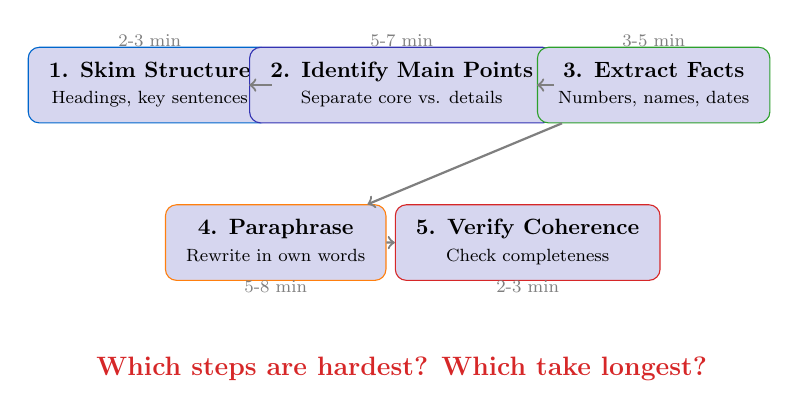
\begin{tikzpicture}[scale=0.8, every node/.style={transform shape}]
% Step boxes
\node[draw=mlblue, fill=mllavender4, rounded corners, minimum width=3cm, minimum height=1.2cm] (skim) at (0, 0) {
\begin{tabular}{c}
\textbf{1. Skim Structure}\\
\footnotesize Headings, key sentences
\end{tabular}
};

\node[draw=mlpurple, fill=mllavender4, rounded corners, minimum width=3cm, minimum height=1.2cm] (identify) at (4, 0) {
\begin{tabular}{c}
\textbf{2. Identify Main Points}\\
\footnotesize Separate core vs. details
\end{tabular}
};

\node[draw=mlgreen, fill=mllavender4, rounded corners, minimum width=3cm, minimum height=1.2cm] (extract) at (8, 0) {
\begin{tabular}{c}
\textbf{3. Extract Facts}\\
\footnotesize Numbers, names, dates
\end{tabular}
};

\node[draw=mlorange, fill=mllavender4, rounded corners, minimum width=3cm, minimum height=1.2cm] (paraphrase) at (2, -2.5) {
\begin{tabular}{c}
\textbf{4. Paraphrase}\\
\footnotesize Rewrite in own words
\end{tabular}
};

\node[draw=mlred, fill=mllavender4, rounded corners, minimum width=3cm, minimum height=1.2cm] (verify) at (6, -2.5) {
\begin{tabular}{c}
\textbf{5. Verify Coherence}\\
\footnotesize Check completeness
\end{tabular}
};

% Arrows
\draw[->, thick, mlgray] (skim) -- (identify);
\draw[->, thick, mlgray] (identify) -- (extract);
\draw[->, thick, mlgray] (extract) -- (paraphrase);
\draw[->, thick, mlgray] (paraphrase) -- (verify);

% Time annotations
\node[above of=skim, yshift=-0.3cm, mlgray] {\footnotesize 2-3 min};
\node[above of=identify, yshift=-0.3cm, mlgray] {\footnotesize 5-7 min};
\node[above of=extract, yshift=-0.3cm, mlgray] {\footnotesize 3-5 min};
\node[below of=paraphrase, yshift=0.3cm, mlgray] {\footnotesize 5-8 min};
\node[below of=verify, yshift=0.3cm, mlgray] {\footnotesize 2-3 min};

% Central question
\node[text=mlred, font=\large\bfseries] at (4, -4.5) {Which steps are hardest? Which take longest?};
\end{tikzpicture}
\end{center}

\bottomnote{Experts develop mental shortcuts, but still limited by working memory}
\end{frame}

% Slide 4: Human Summarization Process (Detail)
\begin{frame}[t]{Human Strengths vs. Weaknesses}
\begin{columns}[T]
\column{0.48\textwidth}
\textbf{\textcolor{mlgreen}{Human Strengths}}
\begin{itemize}
\item Context understanding
  \begin{itemize}
  \footnotesize
  \item Detect sarcasm, irony
  \item Understand implications
  \end{itemize}
\item Audience adaptation
  \begin{itemize}
  \footnotesize
  \item Technical vs. general
  \item Formal vs. casual
  \end{itemize}
\item Judgment calls
  \begin{itemize}
  \footnotesize
  \item What's truly important
  \item Relevance filtering
  \end{itemize}
\item Cross-reference ability
  \begin{itemize}
  \footnotesize
  \item Connect disparate ideas
  \item Synthesize themes
  \end{itemize}
\end{itemize}

\column{0.48\textwidth}
\textbf{\textcolor{mlred}{Human Weaknesses}}
\begin{itemize}
\item Speed limitations
  \begin{itemize}
  \footnotesize
  \item 15-30 min per document
  \item Cognitive fatigue
  \end{itemize}
\item Consistency issues
  \begin{itemize}
  \footnotesize
  \item Quality varies with mood
  \item Different styles between people
  \end{itemize}
\item Scale problems
  \begin{itemize}
  \footnotesize
  \item Can't process 1000/day
  \item Bottleneck in workflows
  \end{itemize}
\item Bias introduction
  \begin{itemize}
  \footnotesize
  \item Personal interpretation
  \item Selective attention
  \end{itemize}
\end{itemize}
\end{columns}

\vspace{3mm}
\begin{center}
\colorbox{mllavender2}{\parbox{0.8\textwidth}{
\centering
\textbf{Example:} Legal contract summary - Lawyer (\$200/hr) takes 1 hour for 50-page contract.\\
Firm needs 1000/month = \textcolor{mlred}{\textbf{\$200,000/month}} in labor costs!
}}
\end{center}

\bottomnote{Human expertise is valuable but doesn't scale to modern volumes}
\end{frame}

% Slide 5: The Scale Problem
\begin{frame}[t]{The Scale Problem - Volume Requirements}
\begin{center}
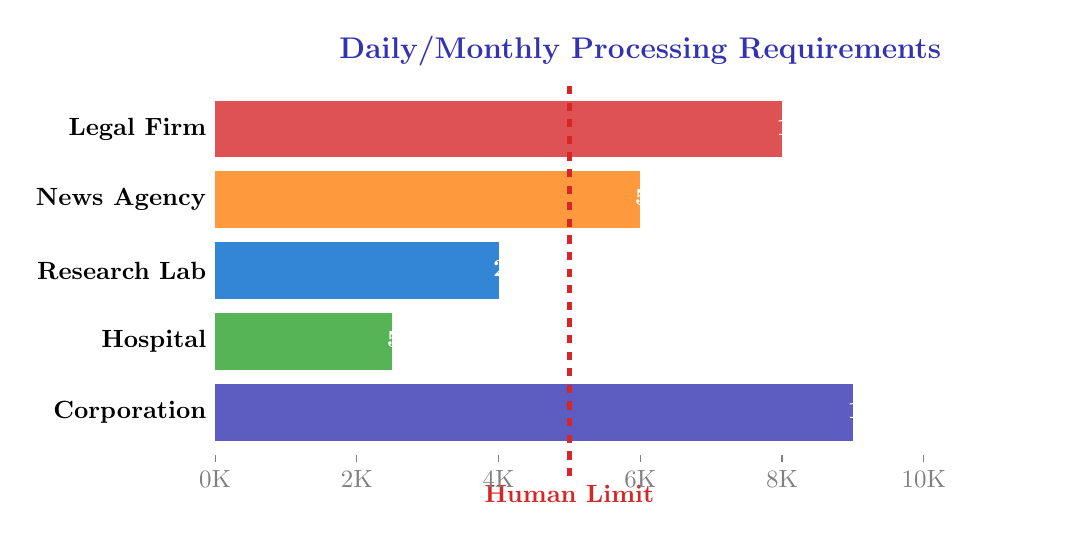
\begin{tikzpicture}[scale=0.9, every node/.style={transform shape}]
% Title
\node[font=\large\bfseries, text=mlpurple] at (6, 5.5) {Daily/Monthly Processing Requirements};

% Bars
\def\barwidth{0.8}
\def\maxlength{10}

% Legal
\fill[mlred!80] (0, 4) rectangle (8, 4+\barwidth);
\node[left] at (0, 4.4) {\textbf{Legal Firm}};
\node[right, white, font=\bfseries] at (7.8, 4.4) {1000 contracts/month};

% News
\fill[mlorange!80] (0, 3) rectangle (6, 3+\barwidth);
\node[left] at (0, 3.4) {\textbf{News Agency}};
\node[right, white, font=\bfseries] at (5.8, 3.4) {500 articles/day};

% Research
\fill[mlblue!80] (0, 2) rectangle (4, 2+\barwidth);
\node[left] at (0, 2.4) {\textbf{Research Lab}};
\node[right, white, font=\bfseries] at (3.8, 2.4) {200 papers/week};

% Hospital
\fill[mlgreen!80] (0, 1) rectangle (2.5, 1+\barwidth);
\node[left] at (0, 1.4) {\textbf{Hospital}};
\node[right, white, font=\bfseries] at (2.3, 1.4) {50 histories/day};

% Corporate
\fill[mlpurple!80] (0, 0) rectangle (9, 0+\barwidth);
\node[left] at (0, 0.4) {\textbf{Corporation}};
\node[right, white, font=\bfseries] at (8.8, 0.4) {10K emails/day};

% Critical line
\draw[dashed, mlred, line width=2pt] (5, -0.5) -- (5, 5);
\node[below, text=mlred] at (5, -0.5) {\textbf{Human Limit}};

% Scale
\foreach \x in {0,2,4,6,8,10} {
  \draw[mlgray] (\x, -0.2) -- (\x, -0.3);
  \node[below, mlgray] at (\x, -0.3) {\x K};
}
\end{tikzpicture}
\end{center}

\vspace{3mm}
\begin{center}
\colorbox{mlred!20}{\parbox{0.9\textwidth}{
\centering
\textbf{Critical Insight:} News agency needs 500 articles × 15 min each = 125 hours/day.\\
Would require \textbf{16 full-time summarizers} working non-stop!
}}
\end{center}

\bottomnote{The bottleneck isn't quality - it's throughput}
\end{frame}

% Slide 6: What Makes a Good Summary?
\begin{frame}[t]{What Makes a Good Summary?}
\begin{columns}[T]
\column{0.55\textwidth}
\begin{center}
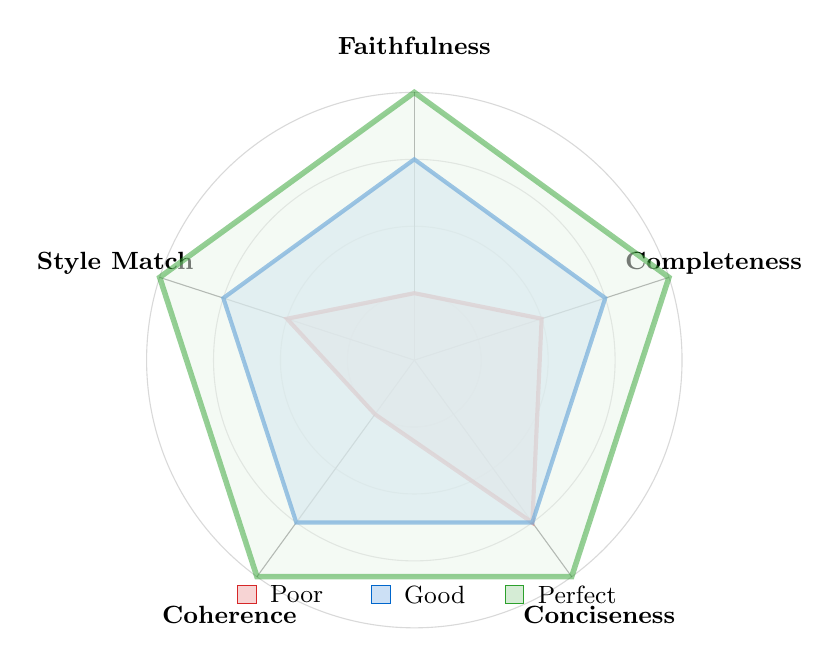
\begin{tikzpicture}[scale=0.85]
% Radar plot setup
\def\numpoints{5}
\def\maxvalue{4}

% Draw grid circles
\foreach \i in {1,...,\maxvalue} {
  \draw[mlgray!30] (0,0) circle (\i);
}

% Draw axes
\foreach \angle/\label in {
  90/Faithfulness,
  18/Completeness,
  -54/Conciseness,
  -126/Coherence,
  162/Style Match} {
  \draw[mlgray] (0,0) -- (\angle:\maxvalue);
  \node[font=\small\bfseries] at (\angle:\maxvalue+0.7) {\label};
}

% Poor summary (red, uneven)
\draw[mlred, line width=1.5pt, fill=mlred!20, opacity=0.7]
  (90:1) -- (18:2) -- (-54:3) -- (-126:1) -- (162:2) -- cycle;

% Good summary (blue, balanced)
\draw[mlblue, line width=1.5pt, fill=mlblue!20, opacity=0.7]
  (90:3) -- (18:3) -- (-54:3) -- (-126:3) -- (162:3) -- cycle;

% Perfect summary (green, outer edge)
\draw[mlgreen, line width=2pt, fill=mlgreen!10, opacity=0.5]
  (90:4) -- (18:4) -- (-54:4) -- (-126:4) -- (162:4) -- cycle;

% Legend
\node[draw=mlred, fill=mlred!20] at (-2.5, -3.5) {};
\node[right] at (-2.3, -3.5) {\small Poor};
\node[draw=mlblue, fill=mlblue!20] at (-0.5, -3.5) {};
\node[right] at (-0.3, -3.5) {\small Good};
\node[draw=mlgreen, fill=mlgreen!20] at (1.5, -3.5) {};
\node[right] at (1.7, -3.5) {\small Perfect};

\end{tikzpicture}
\end{center}

\column{0.43\textwidth}
\textbf{Five Quality Dimensions:}
\begin{enumerate}
\item \textbf{Faithfulness}: No added information
\item \textbf{Completeness}: Key points included
\item \textbf{Conciseness}: Appropriate length
\item \textbf{Coherence}: Natural flow
\item \textbf{Style Match}: Audience-appropriate
\end{enumerate}

\vspace{5mm}
\textbf{Domain Priorities:}
\begin{itemize}
\item \textcolor{mlred}{Legal}: Faithfulness = 100\%
\item \textcolor{mlorange}{News}: Conciseness = 100\%
\item \textcolor{mlgreen}{Medical}: Completeness = 100\%
\end{itemize}

\vspace{3mm}
\textcolor{mlpurple}{\textbf{Question:}} Which dimension matters most? \textit{Depends on use case!}
\end{columns}

\bottomnote{Traditional metrics (ROUGE) only measure overlap, not these qualities}
\end{frame}

% Slide 6.5: Traditional vs. LLM Approaches
\begin{frame}[t]{Evolution of Summarization Techniques}
\begin{center}
\includegraphics[width=0.85\textwidth]{../figures/traditional_vs_llm_matrix_bsc.pdf}
\end{center}

\vspace{-2mm}
\begin{center}
\colorbox{mllavender2}{\parbox{0.85\textwidth}{
\centering
\textbf{Key Insight:} LLMs combine neural understanding with abstractive fluency -\\
they can \textit{understand} the text AND \textit{generate} new summaries, not just extract sentences.
}}
\end{center}

\bottomnote{LLMs succeeded where earlier methods failed by combining the best of both worlds}
\end{frame}

% Slide 7: The Challenge Matrix
\begin{frame}[t]{The Challenge Matrix}
\begin{center}
\begin{tikzpicture}[scale=0.9, every node/.style={transform shape}]
% Grid
\draw[thick, mlgray] (0, 0) rectangle (10, 6);
\draw[thick, mlgray] (5, 0) -- (5, 6);
\draw[thick, mlgray] (0, 3) -- (10, 3);

% Axis labels
\node[font=\large\bfseries] at (5, -0.5) {Document Complexity};
\node[font=\small] at (2.5, -0.5) {Simple};
\node[font=\small] at (7.5, -0.5) {Technical};
\node[font=\large\bfseries, rotate=90] at (-0.5, 3) {Document Length};
\node[font=\small, rotate=90] at (-0.5, 1.5) {Short};
\node[font=\small, rotate=90] at (-0.5, 4.5) {Long};

% Q1: Short/Simple (bottom-left)
\fill[mlgreen!30] (0.2, 0.2) rectangle (4.8, 2.8);
\node[font=\bfseries] at (2.5, 2.3) {News Article};
\node[font=\small] at (2.5, 1.8) {EASY (95\% success)};
\node at (2.5, 1.3) {\includegraphics[width=0.8cm]{../figures/../../common/icons/newspaper.png}};
\node[font=\footnotesize, mlgreen] at (2.5, 0.6) {``Fire in downtown''};

% Q2: Long/Simple (top-left)
\fill[mlorange!30] (0.2, 3.2) rectangle (4.8, 5.8);
\node[font=\bfseries] at (2.5, 5.3) {Wikipedia Page};
\node[font=\small] at (2.5, 4.8) {MEDIUM (80\% success)};
\node at (2.5, 4.3) {\includegraphics[width=0.8cm]{../figures/../../common/icons/wikipedia.png}};
\node[font=\footnotesize, mlorange] at (2.5, 3.6) {``History of Rome''};

% Q3: Short/Technical (bottom-right)
\fill[mlblue!30] (5.2, 0.2) rectangle (9.8, 2.8);
\node[font=\bfseries] at (7.5, 2.3) {Research Abstract};
\node[font=\small] at (7.5, 1.8) {HARD (65\% success)};
\node at (7.5, 1.3) {\includegraphics[width=0.8cm]{../figures/../../common/icons/research.png}};
\node[font=\footnotesize, mlblue] at (7.5, 0.6) {``Quantum entanglement''};

% Q4: Long/Technical (top-right)
\fill[mlred!30] (5.2, 3.2) rectangle (9.8, 5.8);
\node[font=\bfseries] at (7.5, 5.3) {Legal Contract};
\node[font=\small] at (7.5, 4.8) {HARDEST (45\% success)};
\node at (7.5, 4.3) {\includegraphics[width=0.8cm]{../figures/../../common/icons/legal.png}};
\node[font=\footnotesize, mlred] at (7.5, 3.6) {``50-page agreement''};

% Difficulty gradient arrow
\draw[->, ultra thick, mlpurple] (1, 1) -- (9, 5);
\node[mlpurple, font=\small\bfseries, rotate=33] at (5, 2.5) {Increasing Difficulty};

\end{tikzpicture}
\end{center}

\vspace{3mm}
\begin{center}
\textcolor{mlred}{\textbf{Discovery Question:}} What makes some summaries harder than others?
\end{center}

\bottomnote{Different challenges require different prompting strategies}
\end{frame}

% Slide 8: Checkpoint Quiz 1
\begin{frame}[t]{Checkpoint Quiz 1}
\begin{center}
\Large
\textcolor{mlpurple}{\textbf{Question:}}\\[5mm]
\large
Which quality dimension is hardest for\\
automated systems to measure?\\[10mm]
\end{center}

\begin{columns}[T]
\column{0.48\textwidth}
\begin{center}
\huge\textbf{A}\\[3mm]
\large Summary length\\
\normalsize (word count)
\end{center}

\column{0.48\textwidth}
\begin{center}
\huge\textbf{B}\\[3mm]
\large Faithfulness\\
\normalsize (no hallucinations)
\end{center}
\end{columns}

\vspace{8mm}

\begin{columns}[T]
\column{0.48\textwidth}
\begin{center}
\huge\textbf{C}\\[3mm]
\large Compression ratio\\
\normalsize (input/output)
\end{center}

\column{0.48\textwidth}
\begin{center}
\huge\textbf{D}\\[3mm]
\large Word overlap\\
\normalsize (ROUGE score)
\end{center}
\end{columns}

\vspace{10mm}
\pause

\begin{center}
\colorbox{mlgreen!30}{\parbox{0.8\textwidth}{
\centering
\textbf{Answer: B - Faithfulness}\\[2mm]
Length, compression, and overlap are simple math operations.\\
Faithfulness requires understanding semantics and fact-checking against the source.
}}
\end{center}

\bottomnote{This is why we need LLM-based evaluation, not just ROUGE}
\end{frame}

% ============================================================================
% PART 2: TECHNICAL ARCHITECTURE (Slides 9-18)
% ============================================================================

% Slide 9: How Transformers Enable Summarization (Visual)
\begin{frame}[t]{How Transformers Enable Summarization}
\begin{center}
\includegraphics[width=0.75\textwidth]{../figures/attention_mechanism_visual_bsc.pdf}
\end{center}

\vspace{-2mm}
\begin{center}
\colorbox{mllavender2}{\parbox{0.85\textwidth}{
\centering
\textbf{Key Discovery:} Attention mechanism identifies important sentences automatically -\\
Strong weights on: ``1000 patients'', ``5 years'', ``found'' | Weak weights on: ``the'', ``of'', ``over''
}}
\end{center}

\bottomnote{Self-attention learns importance patterns from training data}
\end{frame}

% Slide 10: How Transformers Enable Summarization (Detail)
\begin{frame}[t]{Encoder-Decoder Process}
\begin{columns}[T]
\column{0.48\textwidth}
\textbf{\textcolor{mlblue}{Encoder (Understanding)}}
\begin{itemize}
\item Input tokens → embeddings
\item Self-attention layers (6-12)
\item Learn document structure
\item Identify salient information
\item Output: Encoded representations
\end{itemize}

\vspace{5mm}
\textbf{Example Input:}\\
\footnotesize
``Complex study findings with\\
statistical significance p<0.01...''

\column{0.48\textwidth}
\textbf{\textcolor{mlgreen}{Decoder (Generation)}}
\begin{itemize}
\item Start with [CLS] token
\item Cross-attend to encoder
\item Generate tokens autoregressively
\item Stop at [SEP] or max length
\item Output: Summary tokens
\end{itemize}

\vspace{5mm}
\textbf{Example Output:}\\
\footnotesize
``Study shows significant\\
results (p<0.01)''
\end{columns}

\vspace{5mm}
\begin{center}

\begin{tikzpicture}[scale=0.8]
\draw[->, ultra thick, mlpurple] (0,0) -- (3,0);
\node[above] at (1.5, 0.2) {\small Encoder → Decoder flow};
\end{tikzpicture}
\end{center}

\vspace{3mm}
\textcolor{mlred}{\textbf{Key:}} Decoder can \textit{rephrase}, not just copy!

\bottomnote{Encoder-decoder architecture (BART, T5) vs. decoder-only (GPT, Claude)}
\end{frame}

% Slide 11: Tokenization for Summarization
\begin{frame}[t]{Text to Tokens Pipeline}
\begin{center}
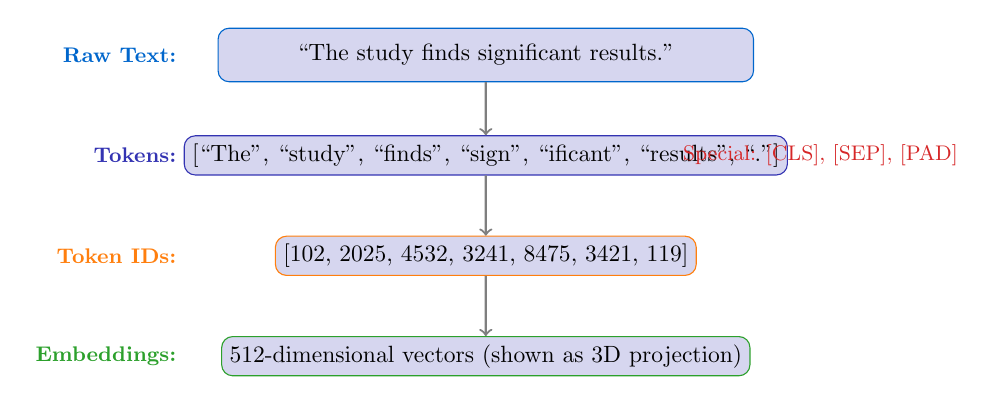
\begin{tikzpicture}[scale=0.85, every node/.style={transform shape}]
% Stage 1: Raw text
\node[draw=mlblue, fill=mllavender4, rounded corners, minimum width=8cm, minimum height=0.8cm] (text) at (0, 4) {
``The study finds significant results.''
};
\node[left, mlblue, font=\small\bfseries] at (-4.5, 4) {Raw Text:};

% Stage 2: Tokens
\node[draw=mlpurple, fill=mllavender4, rounded corners] (tokens) at (0, 2.5) {
[``The'', ``study'', ``finds'', ``sign'', ``ificant'', ``results'', ``.'']
};
\node[left, mlpurple, font=\small\bfseries] at (-4.5, 2.5) {Tokens:};

% Stage 3: Token IDs
\node[draw=mlorange, fill=mllavender4, rounded corners] (ids) at (0, 1) {
[102, 2025, 4532, 3241, 8475, 3421, 119]
};
\node[left, mlorange, font=\small\bfseries] at (-4.5, 1) {Token IDs:};

% Stage 4: Embeddings
\node[draw=mlgreen, fill=mllavender4, rounded corners] (embeddings) at (0, -0.5) {
512-dimensional vectors (shown as 3D projection)
};
\node[left, mlgreen, font=\small\bfseries] at (-4.5, -0.5) {Embeddings:};

% Arrows
\draw[->, thick, mlgray] (text) -- (tokens);
\draw[->, thick, mlgray] (tokens) -- (ids);
\draw[->, thick, mlgray] (ids) -- (embeddings);

% Special tokens highlight
\node[mlred, font=\small] at (5, 2.5) {Special: [CLS], [SEP], [PAD]};
\end{tikzpicture}
\end{center}

\vspace{5mm}
\begin{center}
\colorbox{mlorange!20}{\parbox{0.85\textwidth}{
\centering
\textbf{Why split ``significant'' into ``sign'' + ``ificant''?}\\
Rare word: ``immunotherapy'' → [``immuno'', ``therapy''] (subword units)\\
Benefit: Vocabulary of 30K handles millions of words
}}
\end{center}

\bottomnote{BPE/WordPiece balance vocabulary size vs. coverage}
\end{frame}

% Slide 12: From Understanding to Generation
\begin{frame}[t]{Complete Pipeline with Concrete Numbers}
\begin{center}
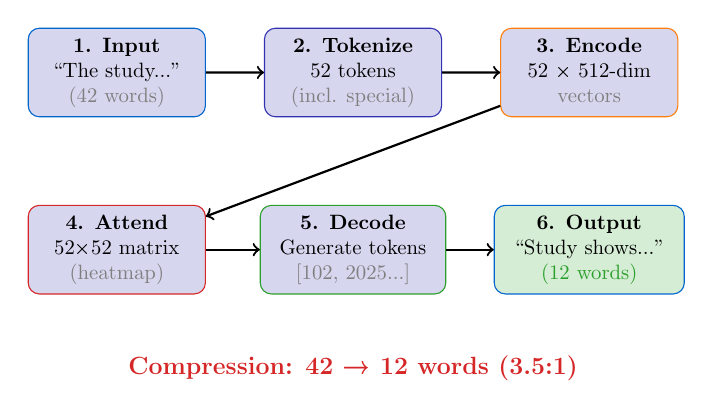
\begin{tikzpicture}[scale=0.75, every node/.style={transform shape}]
% Pipeline boxes
\node[draw=mlblue, fill=mllavender4, rounded corners, minimum width=3cm] (input) at (0, 3) {
\begin{tabular}{c}
\textbf{1. Input}\\
``The study...''\\
\textcolor{mlgray}{(42 words)}
\end{tabular}
};

\node[draw=mlpurple, fill=mllavender4, rounded corners, minimum width=3cm] (tokenize) at (4, 3) {
\begin{tabular}{c}
\textbf{2. Tokenize}\\
52 tokens\\
\textcolor{mlgray}{(incl. special)}
\end{tabular}
};

\node[draw=mlorange, fill=mllavender4, rounded corners, minimum width=3cm] (encode) at (8, 3) {
\begin{tabular}{c}
\textbf{3. Encode}\\
52 × 512-dim\\
\textcolor{mlgray}{vectors}
\end{tabular}
};

\node[draw=mlred, fill=mllavender4, rounded corners, minimum width=3cm] (attend) at (0, 0) {
\begin{tabular}{c}
\textbf{4. Attend}\\
52×52 matrix\\
\textcolor{mlgray}{(heatmap)}
\end{tabular}
};

\node[draw=mlgreen, fill=mllavender4, rounded corners, minimum width=3cm] (decode) at (4, 0) {
\begin{tabular}{c}
\textbf{5. Decode}\\
Generate tokens\\
\textcolor{mlgray}{[102, 2025...]}
\end{tabular}
};

\node[draw=mlblue, fill=mlgreen!20, rounded corners, minimum width=3cm] (output) at (8, 0) {
\begin{tabular}{c}
\textbf{6. Output}\\
``Study shows...''\\
\textcolor{mlgreen}{(12 words)}
\end{tabular}
};

% Arrows
\draw[->, thick] (input) -- (tokenize);
\draw[->, thick] (tokenize) -- (encode);
\draw[->, thick] (encode) -- (attend);
\draw[->, thick] (attend) -- (decode);
\draw[->, thick] (decode) -- (output);

% Compression highlight
\node[mlred, font=\large\bfseries] at (4, -2) {Compression: 42 → 12 words (3.5:1)};
\end{tikzpicture}
\end{center}

\vspace{3mm}
\textbf{Where does compression happen?}\\
Attention focuses on: ``study'', ``shows'', ``significant'', ``results''\\
Ignored: ``the'', ``of'', ``over the course of'', etc.

\bottomnote{Each step is learned from data, not programmed - no rules!}
\end{frame}

% Slide 13: Model Architecture Comparison (Visual)
\begin{frame}[t]{Model Architecture Comparison}
\begin{center}
\includegraphics[width=0.85\textwidth]{../figures/model_architecture_comparison_bsc.pdf}
\end{center}

\vspace{3mm}
\begin{center}
\colorbox{mllavender2}{\parbox{0.85\textwidth}{
\centering
\textbf{Example Use Cases:}\\
News summaries (short, high volume) → FLAN-T5\\
Legal contracts (long, accuracy critical) → Claude
}}
\end{center}

\bottomnote{Choose based on requirements: quality, cost, length, speed}
\end{frame}

% Slide 14: Model Selection Decision Tree
\begin{frame}[t]{Model Selection Decision Tree}
\begin{center}
\includegraphics[width=0.85\textwidth]{../figures/model_selection_decision_tree_bsc.pdf}
\end{center}

\vspace{3mm}
\textbf{Walk through for your use case:}
\begin{itemize}
\item Legal contract: Long (>32K), critical → Claude + RAG + human review
\item News article: Short (<1K), volume → FLAN-T5 batch processing
\end{itemize}

\bottomnote{Combine models: FLAN-T5 for draft, GPT-4 for refinement}
\end{frame}

% Slide 15: Context Window Limits
\begin{frame}[t]{Context Window Limits}
\begin{center}
\includegraphics[width=0.85\textwidth]{../figures/context_window_limits_bsc.pdf}
\end{center}

\vspace{3mm}
\textcolor{mlred}{\textbf{Problem:}} What happens when document exceeds limit?
\begin{itemize}
\item Option 1: Truncate (lose info) ← \textcolor{mlred}{Bad}
\item Option 2: Chunk and summarize separately ← \textcolor{mlgreen}{Good (Part 3)}
\end{itemize}

\bottomnote{Context limits force us to use advanced techniques}
\end{frame}

% Slide 16: Worked Example - Token Flow
\begin{frame}[t]{Worked Example: Token Flow}
\small
\textbf{Input (32 words):}\\
``A recent study examined 1,000 patients with Type 2 diabetes over a 5-year period. The results showed a 30\% reduction in complications for those following the new treatment protocol.''

\vspace{3mm}
\begin{columns}[T]
\column{0.48\textwidth}
\textbf{Tokenization:}\\
\footnotesize
Token IDs: [102, 138, 2332, 4521, 1000, ...]\\
\textcolor{mlgray}{(First 5 of ~40 tokens shown)}

\vspace{3mm}
\textbf{Attention Focus:}\\
\footnotesize
Strong weights on:\\
\textcolor{mlred}{``1,000''}, \textcolor{mlred}{``patients''}, \textcolor{mlred}{``5-year''},\\
\textcolor{mlred}{``30\%''}, \textcolor{mlred}{``reduction''}, \textcolor{mlred}{``complications''}

\column{0.48\textwidth}
\textbf{Generation:}\\
\footnotesize
Output tokens: [102, 2025, 4532, ...]\\
\textcolor{mlgray}{(Decoded to text below)}

\vspace{3mm}
\textbf{Final Output (17 words):}\\
\footnotesize
``Study of 1,000 diabetes patients found 30\% reduction in complications with new treatment over 5 years.''
\end{columns}

\vspace{5mm}
\begin{center}
\begin{tabular}{lccc}
\toprule
\textbf{Metric} & \textbf{Value} & \textbf{Quality} \\
\midrule
Compression & 32 → 17 words (53\%) & \checkmark \\
Faithfulness & All numbers correct & \checkmark \\
Coherence & Grammatical, flows well & \checkmark \\
\bottomrule
\end{tabular}
\end{center}

\bottomnote{This is abstractive summarization - paraphrasing, not copying}
\end{frame}

% Slide 17: Checkpoint Quiz 2
\begin{frame}[t]{Checkpoint Quiz 2}
\begin{center}
\Large
\textcolor{mlpurple}{\textbf{Question:}}\\[5mm]
\large
You have a 50-page legal document (~40K words)\\
and want to use GPT-3.5 (4K token limit).\\
What should you do?\\[10mm]
\end{center}

\begin{columns}[T]
\column{0.48\textwidth}
\begin{center}
\huge\textbf{A}\\[3mm]
\large It will automatically\\compress the input
\end{center}

\column{0.48\textwidth}
\begin{center}
\huge\textbf{B}\\[3mm]
\large The model will\\fail with an error
\end{center}
\end{columns}

\vspace{8mm}

\begin{columns}[T]
\column{0.48\textwidth}
\begin{center}
\huge\textbf{C}\\[3mm]
\large Use chunking\\strategies
\end{center}

\column{0.48\textwidth}
\begin{center}
\huge\textbf{D}\\[3mm]
\large Switch to Claude\\(100K context)
\end{center}
\end{columns}

\vspace{8mm}
\pause

\begin{center}
\colorbox{mlgreen!30}{\parbox{0.8\textwidth}{
\centering
\textbf{Answer: C or D (both valid!)}\\[2mm]
C: Chunk into 10 pieces, summarize each, combine (map-reduce)\\
D: Use Claude if budget allows (simpler but costlier)
}}
\end{center}

\bottomnote{This transition leads us to advanced techniques}
\end{frame}

% Slide 18: Transition - Beyond Basic Prompting
\begin{frame}[t]{Beyond Basic Prompting - Error Distribution}
\begin{columns}[T]
\column{0.55\textwidth}
\begin{center}
\begin{tikzpicture}[scale=0.8]
\pie[
  text=legend,
  radius=3,
  color={mlred!80, mlorange!80, mlblue!80, mlpurple!80, mlgreen!80}
]{
  35/Hallucinations,
  20/Missing Info,
  15/Length Issues,
  20/Style Mismatch,
  10/Factual Errors
}
\end{tikzpicture}
\end{center}

\column{0.43\textwidth}
\textbf{Common Failures:}
\begin{itemize}
\item \textcolor{mlred}{35\% Hallucinations}\\
  \footnotesize Adding fake information
\item \textcolor{mlorange}{20\% Missing Info}\\
  \footnotesize Omitting key points
\item \textcolor{mlblue}{15\% Length Issues}\\
  \footnotesize Too short/long
\item \textcolor{mlpurple}{20\% Style Problems}\\
  \footnotesize Wrong formality
\item \textcolor{mlgreen}{10\% Factual Errors}\\
  \footnotesize Wrong numbers
\end{itemize}

\vspace{5mm}
\textbf{Example Hallucination:}\\
\footnotesize
Input: ``Study of 100 patients...''\\
Output: ``Study of \textcolor{mlred}{1,000} patients showed \textcolor{mlred}{FDA approval}...''
\end{columns}

\vspace{3mm}
\begin{center}
\colorbox{mlred!20}{\parbox{0.85\textwidth}{
\centering
\textbf{With basic prompting, 35\% have hallucinations - Unacceptable!}\\
Need advanced techniques: few-shot, CoT, RAG to fix these
}}
\end{center}

\bottomnote{Need advanced techniques to handle these failure modes}
\end{frame}

% ============================================================================
% PART 3: ADVANCED TECHNIQUES (Slides 19-28)
% ============================================================================

% Slide 19: Prompting Strategies Overview
\begin{frame}[t]{Prompting Strategies - Sophistication Ladder}
\begin{center}
\begin{tikzpicture}[scale=0.9, every node/.style={transform shape}]
% Draw stairs
\foreach \i/\level/\effort/\quality/\use/\color in {
  0/{Zero-Shot}/Low/{60-70\%}/{Simple docs}/mlblue,
  1/{Few-Shot}/Medium/{75-85\%}/{Consistent style}/mlpurple,
  2/{Chain-of-Thought}/{Med-High}/{80-90\%}/{Complex reasoning}/mlorange,
  3/{RAG-Enhanced}/High/{90-95\%}/{Critical accuracy}/mlgreen
} {
  % Step
  \fill[\color!30] (2*\i, \i) rectangle (2*\i+2, \i+1);
  \draw[\color, line width=2pt] (2*\i, \i) rectangle (2*\i+2, \i+1);

  % Level name
  \node[\color, font=\bfseries] at (2*\i+1, \i+0.5) {\level};

  % Properties
  \node[below, font=\footnotesize] at (2*\i+1, \i-0.1) {Effort: \effort};
  \node[below, font=\footnotesize, \color] at (2*\i+1, \i-0.4) {Quality: \quality};
  \node[below, font=\footnotesize, mlgray] at (2*\i+1, \i-0.7) {\use};
}

% Quality arrow
\draw[->, ultra thick, mlred] (-0.5, -0.2) -- (7.5, 3.8);
\node[mlred, rotate=26, font=\small\bfseries] at (3.5, 1.5) {Increasing Quality \& Complexity};

% Title
\node[font=\large\bfseries] at (4, 5) {Start Simple, Add Complexity Only When Needed};
\end{tikzpicture}
\end{center}

\vspace{8mm}
\begin{center}
\textbf{Examples:} News article → Level 1-2 sufficient | Medical record → Level 4 required
\end{center}

\bottomnote{Don't over-engineer - match technique to requirements}
\end{frame}

% Slide 20: Zero-Shot Prompting (Visual)
\begin{frame}[t]{Zero-Shot Prompting}
\begin{center}
\includegraphics[width=0.75\textwidth]{../figures/zero_shot_prompt_bsc.pdf}
\end{center}

\vspace{3mm}
\textbf{When does this work? When does it fail?}
\begin{columns}[T]
\column{0.48\textwidth}
\textcolor{mlgreen}{\textbf{Works well:}}\\
\footnotesize
``Summarize this news article''\\
(common pattern in training)

\column{0.48\textwidth}
\textcolor{mlred}{\textbf{Fails:}}\\
\footnotesize
``Summarize this patent application''\\
(unusual format, rare in training)
\end{columns}

\bottomnote{Zero-shot works for common domains, struggles with specialized ones}
\end{frame}

% Slide 21: Few-Shot Prompting (Detail)
\begin{frame}[t]{Few-Shot Prompting - Teaching by Example}
\begin{center}
\includegraphics[width=0.75\textwidth]{../figures/few_shot_prompt_bsc.pdf}
\end{center}

\vspace{3mm}
\begin{center}
\colorbox{mllavender2}{\parbox{0.85\textwidth}{
\centering
\textbf{Key Insight:} Examples teach length, style, and format\\
With examples: Summaries match desired length (100 words ± 10)\\
Without: Wide variation (50-300 words)
}}
\end{center}

\bottomnote{3-5 examples typically optimal (more = diminishing returns + cost)}
\end{frame}

% Slide 22: Chain-of-Thought Summarization (Visual)
\begin{frame}[t]{Chain-of-Thought Summarization}
\begin{center}
\includegraphics[width=0.8\textwidth]{../figures/cot_summarization_process_bsc.pdf}
\end{center}

\vspace{2mm}
\textbf{Does explicit reasoning improve quality?}\\
\footnotesize
Without CoT: Might miss ``randomized'' (key methodology detail)\\
With CoT: Forces systematic extraction of all components\\
\textcolor{mlgreen}{Result: CoT reduces omissions by ~30\% but increases tokens (cost)}

\bottomnote{CoT trades computation cost for quality improvement}
\end{frame}

% Slide 23: Chain-of-Thought Variants (2024-2025)
\begin{frame}[t]{Chain-of-Thought Variants - Latest Research}
\begin{center}
\includegraphics[width=0.85\textwidth]{../figures/cot_variants_comparison_2024_bsc.pdf}
\end{center}

\vspace{3mm}
\textbf{Which variant for medical summaries?}\\
Answer: \textcolor{mlgreen}{\textbf{Faithful CoT}} - Verifies each claim against source\\
\footnotesize
Step 1: ``Patient is 45-year-old male'' ← verify in source \checkmark\\
Step 2: ``Diagnosed with diabetes'' ← verify in source \checkmark\\
If verification fails → flag for human review

\bottomnote{Variants from recent research (2024-2025), not yet in all APIs}
\end{frame}

% Slide 24: RAG-Enhanced Summarization (Visual)
\begin{frame}[t]{RAG-Enhanced Summarization}
\begin{center}
\includegraphics[width=0.8\textwidth]{../figures/rag_summarization_pipeline_bsc.pdf}
\end{center}

\vspace{2mm}
\textcolor{mlpurple}{\textbf{Why retrieve if summarizing the whole document?}}\\
\footnotesize
• Long document (100 pages): Can't fit in context\\
• Query-focused: ``Summarize sections about side effects''\\
• RAG retrieves: Only relevant chunks (pages 23, 45, 67, 89)\\
• Result: Focused summary instead of generic overview

\bottomnote{RAG reduces hallucinations by 40-60\% with proper implementation}
\end{frame}

% Slide 25: RAG-Enhanced Summarization (Detail)
\begin{frame}[t]{When and How to Use RAG}
\begin{columns}[T]
\column{0.48\textwidth}
\textbf{When to Use RAG:}
\begin{itemize}
\item Multi-document summarization
\item Factual domains (medical, legal)
\item Citation tracking needed
\item Very long documents (>context)
\item Query-focused summaries
\end{itemize}

\vspace{5mm}
\textbf{RAG Components:}
\begin{itemize}
\item Embedding model (sentence-transformers)
\item Vector database (FAISS, Pinecone)
\item Retriever (BM25, dense retrieval)
\item Reranker (Cross-encoder)
\item Generator (GPT-4, Claude)
\end{itemize}

\column{0.48\textwidth}
\textbf{Example - Medical Paper:}\\
\footnotesize
\textbf{Input:} 30-page paper + 50 cited papers\\[2mm]
\textbf{Without RAG:}\\
``Paper discusses treatment...'' (generic)\\[2mm]
\textbf{With RAG:}\\
``Paper shows 30\% improvement (Smith 2020), confirmed by Jones 2021, contradicts Brown 2019...''\\[2mm]
\textcolor{mlgreen}{Value: Verifiable, grounded}

\vspace{5mm}
\begin{center}
\colorbox{mlorange!20}{\parbox{0.95\textwidth}{
\centering
\footnotesize
\textbf{Trade-off:} RAG adds complexity\\
Worth it for critical applications
}}
\end{center}
\end{columns}

\bottomnote{Requires infrastructure (vector DB) but essential for critical applications}
\end{frame}

% Slide 26: Handling Long Documents
\begin{frame}[t]{Three Strategies for Long Documents}
\begin{columns}[T]
\column{0.32\textwidth}
\textbf{Map-Reduce}\\
\includegraphics[width=\textwidth]{../figures/map_reduce_summarization_bsc.pdf}\\
\footnotesize
\checkmark~Parallelizable\\
\checkmark~Preserves structure\\
$\times$~May lose cross-chunk connections

\column{0.32\textwidth}
\textbf{Recursive Hierarchical}\\
\includegraphics[width=\textwidth]{../figures/recursive_hierarchical_bsc.pdf}\\
\footnotesize
\checkmark~Handles any length\\
\checkmark~Maintains hierarchy\\
$\times$~Slow, iterative

\column{0.32\textwidth}
\textbf{Sliding Window}\\
\begin{center}
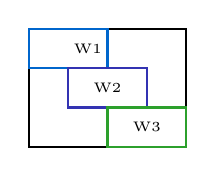
\begin{tikzpicture}[scale=0.5]
% Document
\draw[thick] (0,0) rectangle (4,3);
% Windows
\draw[mlblue, thick] (0,2) rectangle (2,3);
\draw[mlpurple, thick] (1,1) rectangle (3,2);
\draw[mlgreen, thick] (2,0) rectangle (4,1);
% Overlap
\node[font=\tiny] at (1.5, 2.5) {W1};
\node[font=\tiny] at (2, 1.5) {W2};
\node[font=\tiny] at (3, 0.5) {W3};
\end{tikzpicture}
\end{center}
\footnotesize
\checkmark~Catches cross-boundary\\
\checkmark~Flexible coverage\\
$\times$~Complex to implement
\end{columns}

\vspace{5mm}
\begin{center}
\textbf{Which strategy for a 100-page report?}\\
Answer: Map-Reduce for speed (parallel) | Risk: Miss connections between chapters
\end{center}

\bottomnote{Choice depends on document structure - narrative vs. sectioned}
\end{frame}

% Slide 27: Worked Example - Map-Reduce
\begin{frame}[t]{Worked Example: Map-Reduce in Action}
\footnotesize
\textbf{Input:} 20-page research report

\vspace{3mm}
\begin{columns}[T]
\column{0.3\textwidth}
\textbf{Stage 1: Split}\\
\footnotesize
\colorbox{mlblue!20}{Pages 1-4: Intro}\\
\colorbox{mlpurple!20}{Pages 5-8: Methods}\\
\colorbox{mlorange!20}{Pages 9-12: Results}\\
\colorbox{mlgreen!20}{Pages 13-16: Discussion}\\
\colorbox{mlred!20}{Pages 17-20: Conclusion}

\column{0.35\textwidth}
\textbf{Stage 2: Map (Summarize)}\\
\footnotesize
→ ``Report introduces...''\\
→ ``Methods include RCT...''\\
→ ``Results show 30\%...''\\
→ ``Discussion highlights...''\\
→ ``Conclusion recommends...''\\[2mm]
\textcolor{mlgray}{5 summaries × 100 words = 500 words total}

\column{0.33\textwidth}
\textbf{Stage 3: Reduce (Combine)}\\
\footnotesize
\colorbox{mlgreen!20}{\parbox{\textwidth}{
``Report on treatment effectiveness. RCT of 1,000 patients showed 30\% reduction. Despite limitations, adoption recommended.''
}}\\[2mm]
\textcolor{mlgray}{Final: 50 words}
\end{columns}

\vspace{5mm}
\begin{center}
\begin{tabular}{lcc}
\toprule
\textbf{Stage} & \textbf{Words} & \textbf{Tokens} \\
\midrule
Input & 10,000 & ~13,000 \\
After Map & 500 & ~650 \\
After Reduce & 50 & ~65 \\
\bottomrule
\end{tabular}
\end{center}

\textbf{Compression ratio:} 13,000 → 65 = \textcolor{mlred}{\textbf{200:1}}

\bottomnote{Preserves structure but may lose connections between sections}
\end{frame}

% Slide 28: Checkpoint Quiz 3
\begin{frame}[t]{Checkpoint Quiz 3}
\begin{center}
\Large
\textcolor{mlpurple}{\textbf{Question:}}\\[5mm]
\large
You need to summarize a 100-page legal contract\\
where clauses reference each other across sections.\\
Which technique should you use?\\[10mm]
\end{center}

\begin{columns}[T]
\column{0.48\textwidth}
\begin{center}
\huge\textbf{A}\\[3mm]
\large Zero-shot prompting\\
\normalsize (simple)
\end{center}

\column{0.48\textwidth}
\begin{center}
\huge\textbf{B}\\[3mm]
\large Few-shot prompting\\
\normalsize (with examples)
\end{center}
\end{columns}

\vspace{8mm}

\begin{columns}[T]
\column{0.48\textwidth}
\begin{center}
\huge\textbf{C}\\[3mm]
\large RAG with\\citation tracking
\end{center}

\column{0.48\textwidth}
\begin{center}
\huge\textbf{D}\\[3mm]
\large Map-reduce with\\overlap + CoT
\end{center}
\end{columns}

\vspace{5mm}
\pause

\begin{center}
\colorbox{mlgreen!30}{\parbox{0.85\textwidth}{
\centering
\textbf{Answer: D (best) or C (acceptable)}\\[2mm]
A/B: Won't fit in context (contract too long)\\
C: RAG good for retrieval, but might miss cross-references\\
D: Overlap captures cross-references, CoT ensures reasoning\\
\textbf{Optimal:} Combine D + C (map-reduce with RAG for verification)
}}
\end{center}

\bottomnote{Real production systems often stack multiple techniques}
\end{frame}

% ============================================================================
% PART 4: EVALUATION & PRACTICE (Slides 29-35)
% ============================================================================

\section{Evaluation \& Practice}

% Slide 29: Evaluation Metrics Overview (pyramid)
\begin{frame}[t]{How Do We Measure Success?}
\begin{columns}[T]
\column{0.48\textwidth}
\begin{center}
\includegraphics[width=0.95\textwidth]{../figures/evaluation_metrics_bsc.pdf}
\end{center}

\column{0.48\textwidth}
\textbf{The Evaluation Pyramid}

\textbf{Level 1: Surface Metrics}
\begin{itemize}
\item Length compliance
\item Format checking
\item Speed/cost
\end{itemize}

\textbf{Level 2: Content Metrics}
\begin{itemize}
\item ROUGE scores (overlap)
\item BERTScore (semantic)
\item Factuality checks
\end{itemize}

\textbf{Level 3: Quality Metrics}
\begin{itemize}
\item Human evaluation
\item LLM-as-judge
\item Task-specific measures
\end{itemize}
\end{columns}

\bottomnote{Good evaluation requires multiple metrics at different levels}
\end{frame}

% Slide 30: ROUGE Explained (with calculation example)
\begin{frame}[t]{ROUGE: The Classic Metric}
\begin{columns}[T]
\column{0.48\textwidth}
\textbf{ROUGE-N Calculation}

\textbf{Reference:}\\
``The cat sat on the mat''

\textbf{Summary:}\\
``The cat on mat''

\vspace{3mm}
\textbf{ROUGE-1 (unigrams):}
\begin{itemize}
\item Overlap: \{the, cat, on, mat\}
\item Precision: 4/4 = 1.0
\item Recall: 4/6 = 0.67
\item F1: 2×(1.0×0.67)/(1.0+0.67) = 0.80
\end{itemize}

\textbf{ROUGE-2 (bigrams):}
\begin{itemize}
\item Reference: \{the cat, cat sat, sat on, on the, the mat\}
\item Summary: \{the cat, cat on, on mat\}
\item Overlap: \{the cat\}
\item Recall: 1/5 = 0.20
\end{itemize}

\column{0.48\textwidth}
\textbf{ROUGE Variants}

\begin{center}
\begin{tabular}{ll}
\toprule
\textbf{Metric} & \textbf{Measures} \\
\midrule
ROUGE-1 & Unigram overlap \\
ROUGE-2 & Bigram overlap \\
ROUGE-L & Longest sequence \\
ROUGE-S & Skip-bigrams \\
\bottomrule
\end{tabular}
\end{center}

\vspace{5mm}
\textbf{Pros:}
\begin{itemize}
\item Fast to compute
\item Language-agnostic
\item Interpretable
\end{itemize}

\textbf{Cons:}
\begin{itemize}
\item Surface-level only
\item Ignores semantics
\item Prefers extractive
\end{itemize}
\end{columns}

\bottomnote{ROUGE remains popular despite limitations - always combine with other metrics}
\end{frame}

% Slide 31: Modern Metrics Comparison (using new chart)
\begin{frame}[t]{Modern Evaluation Landscape}
\begin{center}
\includegraphics[width=0.85\textwidth]{../figures/modern_metrics_comparison_2024_bsc.pdf}
\end{center}

\vspace{3mm}
\begin{center}
\textbf{Key Trade-offs:} Cost vs Quality vs Speed

\begin{tabular}{lccc}
\toprule
\textbf{Method} & \textbf{Cost} & \textbf{Quality} & \textbf{Speed} \\
\midrule
ROUGE & Low & Medium & Fast \\
BERTScore & Low & Good & Medium \\
G-eval & Medium & Very Good & Slow \\
Human & High & Best & Very Slow \\
\bottomrule
\end{tabular}
\end{center}

\bottomnote{Choose metrics based on your specific use case and constraints}
\end{frame}

% Slide 32: Common Failure Modes
\begin{frame}[t]{When Things Go Wrong}
\begin{columns}[T]
\column{0.48\textwidth}
\begin{center}
\includegraphics[width=0.95\textwidth]{../figures/hallucination_types_taxonomy_bsc.pdf}
\end{center}

\column{0.48\textwidth}
\textbf{Common Failure Patterns}

\textbf{1. Hallucination (35\%)}
\begin{itemize}
\item Adding facts not in source
\item Example: ``FDA-approved'' when not mentioned
\end{itemize}

\textbf{2. Omission (25\%)}
\begin{itemize}
\item Missing key information
\item Example: Ignoring limitations
\end{itemize}

\textbf{3. Distortion (20\%)}
\begin{itemize}
\item Changing meaning
\item Example: ``may'' → ``will''
\end{itemize}

\textbf{4. Repetition (20\%)}
\begin{itemize}
\item Redundant content
\item Example: Saying same thing 3 ways
\end{itemize}
\end{columns}

\bottomnote{Understanding failure modes helps you design better mitigation strategies}
\end{frame}

% Slide 33: Debugging & Mitigation
\begin{frame}[t]{Debugging Flowchart}
\begin{columns}[T]
\column{0.55\textwidth}
\begin{center}
\includegraphics[width=0.95\textwidth]{../figures/failure_modes_flowchart_bsc.pdf}
\end{center}

\column{0.43\textwidth}
\textbf{Quick Fixes}

\textbf{Too Creative?}
\begin{itemize}
\item Lower temperature (0.3-0.5)
\item Reduce top\_p (0.9)
\item Add ``stick to facts'' prompt
\end{itemize}

\textbf{Too Short?}
\begin{itemize}
\item Add min\_length constraint
\item Prompt: ``comprehensive summary''
\item Use few-shot examples
\end{itemize}

\textbf{Hallucinating?}
\begin{itemize}
\item Add RAG verification
\item Lower temperature to 0.3
\item Post-process fact checking
\end{itemize}

\textbf{Repetitive?}
\begin{itemize}
\item Increase repetition\_penalty
\item Use diverse beam search
\item Post-process deduplication
\end{itemize}
\end{columns}

\bottomnote{Systematic debugging saves hours of frustration - follow the flowchart!}
\end{frame}

% Slide 34: Hands-On Example (complete pipeline)
\begin{frame}[fragile,t]{Complete Pipeline Example}
\begin{columns}[T]
\column{0.48\textwidth}
\textbf{Task:} Summarize research paper (8 pages)

\begin{lstlisting}[language=Python, basicstyle=\tiny\ttfamily]
import openai
from rouge import Rouge

def smart_summarize(text, max_tokens=4000):
    # 1. Check length
    if len(text) > max_tokens:
        # 2. Use map-reduce
        chunks = chunk_with_overlap(
            text,
            chunk_size=3000,
            overlap=500
        )

        # 3. Summarize chunks
        summaries = []
        for chunk in chunks:
            summary = openai.chat.completions.create(
                model="gpt-3.5-turbo",
                messages=[{
                    "role": "system",
                    "content": "Summarize:"
                }, {
                    "role": "user",
                    "content": chunk
                }],
                temperature=0.5,
                max_tokens=300
            )
            summaries.append(summary)

        # 4. Combine summaries
        final_text = " ".join(summaries)
    else:
        final_text = text

    # 5. Final summary with CoT
    return generate_final(final_text)
\end{lstlisting}

\column{0.48\textwidth}
\textbf{Configuration Checklist}

\textbf{Model Selection:}
\begin{itemize}
\item GPT-3.5: Speed/cost priority
\item GPT-4: Quality priority
\item Claude: Long context (100k+)
\end{itemize}

\textbf{Parameters:}
\begin{itemize}
\item temperature: 0.5 (balanced)
\item top\_p: 0.9 (some creativity)
\item max\_tokens: 300 per chunk
\item repetition\_penalty: 1.1
\end{itemize}

\textbf{Quality Checks:}
\begin{itemize}
\item Length: 20-30\% of original
\item ROUGE-L: > 0.35
\item No hallucinations (fact check)
\item Coherent flow
\end{itemize}

\textbf{Result:}\\
\colorbox{mlgreen!30}{8 pages → 1.5 pages}\\
\colorbox{mlgreen!30}{ROUGE-L: 0.42}\\
\colorbox{mlgreen!30}{Human rating: 4.2/5}
\end{columns}

\bottomnote{Production pipelines combine multiple techniques for robustness}
\end{frame}

% Slide 35: Summary & Next Steps
\begin{frame}[t]{What We've Learned}
\begin{columns}[T]
\column{0.32\textwidth}
\textbf{Foundations}
\begin{itemize}
\item Information explosion problem
\item LLMs vs traditional methods
\item Transformer architecture
\item Attention is all you need
\end{itemize}

\vspace{3mm}
\textbf{Key Techniques}
\begin{itemize}
\item Zero/few-shot prompting
\item Chain-of-thought
\item RAG enhancement
\item Map-reduce for scale
\end{itemize}

\column{0.32\textwidth}
\textbf{Best Practices}
\begin{itemize}
\item Start simple (zero-shot)
\item Test systematically
\item Monitor for failures
\item Use multiple metrics
\end{itemize}

\vspace{3mm}
\textbf{Parameters}
\begin{itemize}
\item Temperature: 0.3-0.7
\item Top-p: 0.9
\item Repetition penalty: 1.1
\item Chunk overlap: 10-20\%
\end{itemize}

\column{0.32\textwidth}
\textbf{Next Steps}
\begin{enumerate}
\item Try lab notebook
\item Experiment with prompts
\item Build your pipeline
\item Test on your data
\end{enumerate}

\vspace{3mm}
\textbf{Resources}
\begin{itemize}
\item Lab: \texttt{week\_summarization.ipynb}
\item Charts: 87 PDFs in \texttt{figures/}
\item Scripts: \texttt{python/*.py}
\end{itemize}
\end{columns}

\vspace{5mm}
\begin{center}
\colorbox{mllavender3}{\parbox{0.85\textwidth}{
\centering
\large\textbf{Remember:} LLM summarization is powerful but requires careful configuration.\\
Start simple, iterate based on metrics, and always validate output quality!
}}
\end{center}

\bottomnote{You now have all the tools to build production-ready summarization systems}
\end{frame}

% ============================================================================
% END SLIDE
% ============================================================================

\begin{frame}[plain]
\vfill
\centering
\begin{beamercolorbox}[sep=8pt,center]{title}
\usebeamerfont{title}\Huge Thank You!\\[10pt]
\large Questions \& Discussion\\[20pt]
\normalsize Lab notebooks available in \texttt{NLP\_slides/summarization\_module/lab/}
\end{beamercolorbox}
\vfill
\end{frame}

\end{document}